
\documentclass{article}

\usepackage[utf8]{inputenc}
\usepackage{geometry}
\usepackage{amsmath}
\usepackage{graphicx}
\usepackage{float}

 \geometry{
 a4paper,
 total={170mm,257mm},
 left=20mm,
 top=20mm,
 }

\title{Relatório do trabalho 1}
\date{17/04/2019}
\author{Allan Nozomu Fukasawa RA:163527}

\begin{document}
\twocolumn
\maketitle

\section{Introdução}

O objetivo deste trabalho é implementar alguns filtros de imagens no domínio espacial e de frequência. "A filtragem aplicada a uma imagem digital é uma operação que alter os valores de intensidade dos pixels da imagem levando-se em conta o valor do pixel em questão quanto valores de pixels vizinhos." \cite{Helio:1}

\section{Componentes}

Está sendo enviado junto a este relatório, o arquivo Trabalho 1.ipynb onde contém todo o código executado durante este trabalho, 5 imagens de exemplo (sendo a que está sendo usada no programa é, por padrão, a house.png, Figura \ref{fig:original}.) e uma pasta results contendo todos os resultados finais e intermediários.

\begin{figure}[h!]
    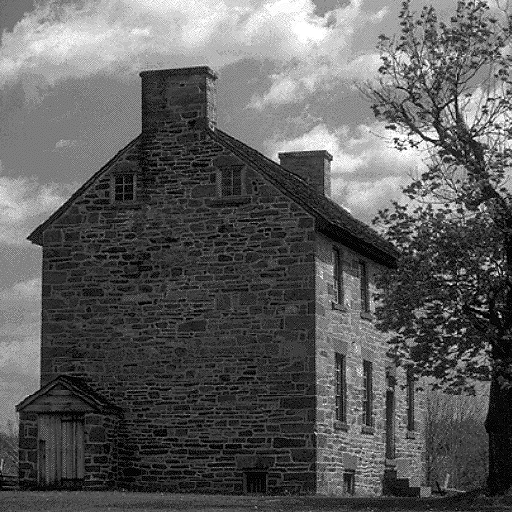
\includegraphics[width=\linewidth]{house.png}
    \caption{Imagem original}
    \label{fig:original}
\end{figure}


\subsection{O Programa}

O programa foi implementado com Jupyter Notebooks, usando Python 3.7.1. As bibliotecas utilizadas no desenvolvimento do programa foram, com suas respectivas versões: 

\begin{itemize}
    \item numpy (1.15.4): para manipulação dos vetores.

    \item matplotlib (3.0.2): visualização dos dados, resultados finais e intermediários.

    \item opencv (3.4.2): realização da leitura e escrita das imagens, transformação das cores e normalização dos dados.

    \item scipy.ndimage (1.1.0): transformações das imagens (Transformada de Fourier e sua inversa), aplicação dos filtros.
\end{itemize}

\subsection{Formato das imagens}

As imagens de entrada e de saída serão no formato PNG (Portable Network Graphics) em tom de cinza. Todas as imagens serão salvas na pasta results para melhor organização do projeto. 

\section{Solução}

\subsection{Leitura das imagens}

A imagem de entrada é lida com função \textbf{cv2.imread} que armazena a imagem em um \textbf{numpy.ndarray} de 3 dimensões (MxNx3).

Depois de lida, a imagem é convertida para níveis de cinza pela função \textbf{cv2.cvtColor} e também tem seus valores convertidos para float, dividindo seu valor por 255, o maior número. Dessa forma, não é necessário se preocupar com overflow e underflow dos números nas operações dos diferentes filtros aplicados.

\subsection{Escrita das imagens}

Também foi feito uma função auxiliar para facilitar na saída das imagens. Antes de tudo, a imagem é normalizada utilizando \textbf{cv2.normalize}, transformando a imagem que antes estava como float em inteiro novamente, variando de 0 a 255.

Após a normalização, a escrita da imagem é feita utilizando a função \textbf{cv2.imwrite} 

Há também algumas imagens salvas a partir do \textbf{matplotlib} correspondente aos resultados das imagens no domínio de frequência. Estas foram salvas utilizando a função \textbf{matplotlib.pyplot.savefig}. 

\subsection{Plotagem das imagens}

Foi utilizado para visualização dos resultados as funções de plotagem de imagens em \textbf{matplotlib.pyplot}, utilizando a paleta de cores em escalas de cinza. Não foi necessário fazer a normalização para a visualização dos dados, porque a função já realiza uma normalização linear.

\subsection{Filtragem em domínio espacial}

Para a aplicação do filtro em domínio espacial utiliza-se uma operação de convolução de uma máscara pela imagem. Este processo é equivalente a percorrer a imagem modificando seus valores conforme os pesos da máscara e as intensidades da imagem. 

Para realizarmos a função de convolução foi utilizado \textbf{ndimage.convolve}. Para o tratamento das bordas, foi feito uma moldura formada por 0, dessa forma, serão ignorados na operação de convolução.

Foi feito um truncamento dos resultados obtidos entre 0 e 255, principalmente nos filtros passa-alta onde valores podem ser muito grandes ou pequenos. Dessa forma, obteu-se uma diferente maneira e também mais fácil na detecção de bordas. Além disso, os valores nessas imagens foram invertidos nesses casos. Desse modo, as bordas se destacariam com a cor preta e o fundo, cor branca.

Ao todo foram feitos 5 filtros: um filtro passa alta, um filtro passa baixa, dois filtros para detecção de borda (horizontal e vertical) e a combinação dos dois anteriores.

\subsubsection{Filtro Laplaciano}

O primeiro filtro aplicado foi um filtro passa-alta conhecido como Filtro Laplaciano. Seu uso mais comum é para detecção de bordas em imagens. O resultado obtido está na Figura \ref{fig:exercicio1a}.

\begin{figure}[h!]
    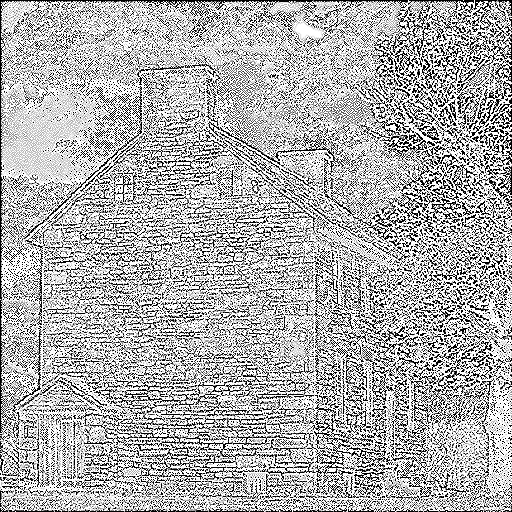
\includegraphics[width=\linewidth]{results/exercicio1aclipada.png}
    \caption{Filtro laplaciano, valores truncados}
    \label{fig:exercicio1a}
\end{figure}

Podemos notar algumas limitações desse algoritmo quanto ao resultado com ruídos, provocados pela imagem original. Para melhores resultados, foi passado antes um filtro que que eliminasse ou diminuísse o ruído (o filtro gaussiano utilizado na segunda parte do exercício) antes de aplicar o filtro laplaciano para detecção de bordas. 

Com isso, temos o seguinte resultado na Figura \ref{fig:exercicio1agauss} . Nota-se uma melhora notável entre as duas imagens principalmente perto do telhado onde a imagem original apesentava bastante ruído e chuviscos.

\begin{figure}[h!]
    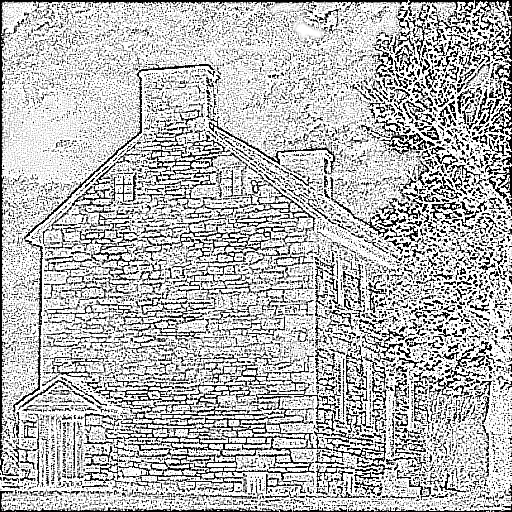
\includegraphics[width=\linewidth]{results/exercicio1agaussiano.png}
    \caption{aplicação do filtro laplaciano após gaussiano}
    \label{fig:exercicio1agauss}
\end{figure}

\subsubsection{Filtro passa-baixa Gaussiano}

O segundo filtro aplicado foi um filtro passa-baixa gaussiano. Seu resultado causa um borramento, muitas vezes utilizado para redução de ruído e detalhamento.

\begin{figure}[h!]
    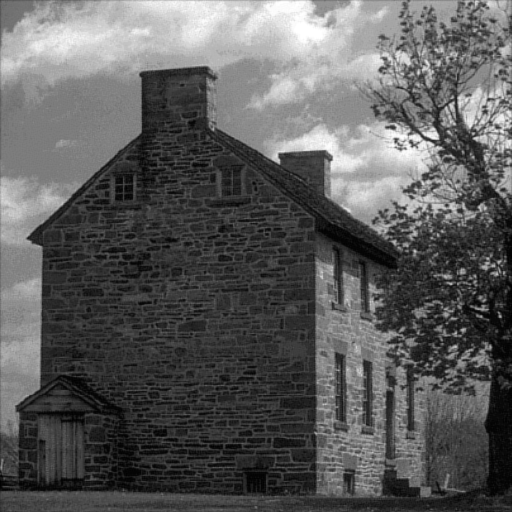
\includegraphics[width=\linewidth]{results/exercicio1b.png}
    \caption{aplicação do filtro passa-baixa gaussiano}
    \label{fig:exercicio1b}
\end{figure}


Por se tratar de um filtro separável, ele foi separado em dois filtros: linha e coluna. Dessa forma, há um ganho computacional pois o número de operações de multipliação será bem menor para cada pixel da imagem. Para a tranforação dos filtros tanto em linha quanto coluna, foi usado a função \textbf{reshape} presentes nos \textbf{numpy.ndarray}.

Depois de realizado a filtragem na linha e coluna, o resultado de ambos foi somado, obtendo a seguinte imagem filtrada (Figura \ref{fig:exercicio1b}). Podemos notar uma redução no ruído (principalmente nas nuvens e também nas janelas da casa).

\subsubsection{Filtro Sobel}

Os três seguintes filtros são os de Sobel, utilizados sobretudo, para detecção de bordas. Dois desses filtros são para calcular as variações verticais e horizontais, logo, cada um deles vai detectar contornos na vertical e horizontal como observados na Figura \ref{fig:exercicio1c}.

\begin{figure}[h!]
    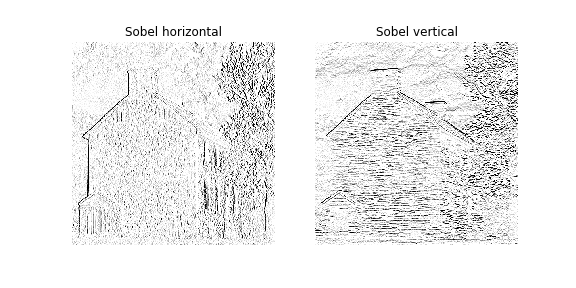
\includegraphics[width=\linewidth]{results/sobelclip.png}
    \caption{Detecção de bordas verticais e horizontais com valores truncados}
    \label{fig:exercicio1c}
\end{figure}

Com ambos os filtros calculados, o filtro resultante de Sobel (magnitude) se dá pela raiz quadrada da soma dos quadrados de cada pixel obtidos anteriormente, resultando na Figura \ref{fig:exercicio1cfinal}.
Podemos notar uma detecção de borda que, apesar do ruído da imagem, apresentou resultados satisfatórios em comparaçõ ao primeiro filtro laplaciano \ref{fig:exercicio1a}.

Comparado ao filtro Laplaciano, este apresentou uma tolerância maior em relação aos ruídos e na detecção de bordas.

\begin{figure}[h!]
    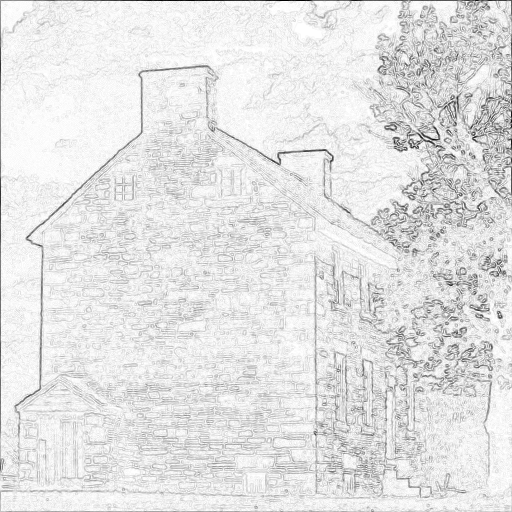
\includegraphics[width=\linewidth]{results/exercicio1c.png}
    \caption{Detecção de bordas po Sobel}
    \label{fig:exercicio1cfinal}
\end{figure}

\subsection{Filtragem domínio de frequência}

Para a aplicação do filtro em domínio de frequência, foi necessário antes de tudo, tranformar a imagem do domínio espacial para o de frequência. Para isso, foi utilziado a função \textbf{numpy.fft.fft2} que implementa a Tranformada Rápida de Fourier (FFT). Também foi feito a translação da frequência zero para o centro do espectro utilizando a função \textbf{numpy.fft.fftshift}.

Foi também realizado um pequeno tratamento para uma melhor compreensão do espectro de frequência. Foi feito uma operação logarítmica \textbf{numpy.log} depois de calculado o valor absoluto do espectro de frequência \textbf{numpy.abs}, obtendo o resultado na \ref{fig:espectro}.

\begin{figure}[h!]
    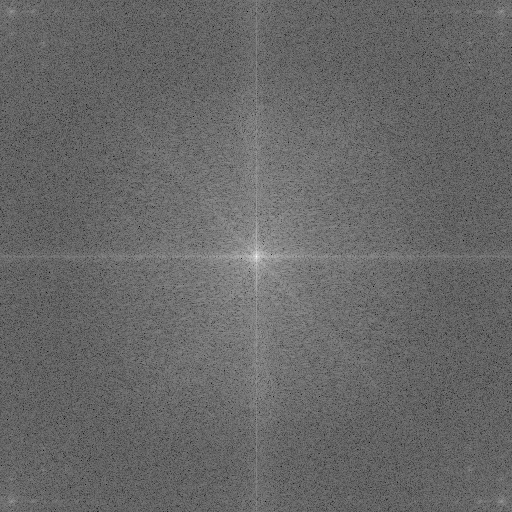
\includegraphics[width=\linewidth]{results/espectro.png}
    \caption{Espectro de frequência}
    \label{fig:espectro}
\end{figure}

Para a aplicação do filtro, basta definirmos uma função de máscara em torno do espectro de frequência que permite a passagem (parcial ou inteira) ou não das faixas de frequência. Filtros passa alta são definidos nas frequências mais altas (nas bordas), enquanto os filtros passa-baixa nas frequências mais ao centro, porque a imagem foi transladada a partir do centro.

Para a contrução da máscara, um \textbf{numpy.array} de indices começando a partir do centro da imagem e crescendo conforme aproximando das bordas foi criado. Dessa forma, foi calculado as distâncias dos filtros.

Para tranformar a imagem de volta para o domínio espacial a partir  do domínio de frequência, após aplicar os filtros, é necessário realizar o processo inverso. É realizado primeiramente a translação da frequência zero utilizando sua inversa \textbf{numpy.fft.ifftshift} e depois a inversa da Tranformada de Fourier \textbf{numpy.fft.ifft2}.

No domínio de frequência, foram realizados 4 diferentes tipos de filtro gausiano: passa-alta, passa-baixa, passa-faixa e rejeita-faixa.

\subsubsection{Passa alta gaussiano}

Para o filtro passa-alta, foram feito 4 filtragens com os respectivos valores de corte: 2, 10, 25 e 200. Conforme o número de corte aumenta, diminui o número de detalher da imagens, permanecendo apenas os contornos.

Em números altos de corte, é impossível distinguir elementos da imagem original, como na frequência de corte 200. O resultado pode ser conferido na Figura \ref{fig:exercicio21}.

\subsubsection{Passa baixa gaussiano}

Para o filtro passa-baixa, foram feito 4 filtragens com os respectivos valores de corte: 10, 25, 100 e 200. Conforme o número de corte diminui, aumenta o nível de borramento da imagem

Em números baixos de corte, a imagem apresenta um borramento muito alto, perdendo o nível de detalhamento da imagem. O resultado pode ser conferido na Figura \ref{fig:exercicio22}.

\subsubsection{Passa faixa gaussiano}

Para o filtro passa-faixa, foram feito 4 filtragens com os respectivos valores em par, tanto para corte quanto para a largura da faixa respectivamente: (25, 50), (50, 100), (100, 200) e (200, 400). 
Tem-se um resultado similar ao filtro passa-alta gaussiano, acentuando os contornos da imagem conforme diminuímos o raio de corte e da largura da faixa. O resultado pode ser conferido na Figura \ref{fig:exercicio23}.

\subsubsection{Rejeita faixa gaussiano}

Para o filtro rejeita-faixa, foram feito 4 filtragens com os respectivos valores em par, tanto para corte quanto para a largura da faixa respectivamente: (25, 50), (50, 100), (100, 200) e (200, 400). 
Tem-se um resultado similar ao filtro passa-baixa gaussiano, apresentando um borramento com efeitos de ruído (chuviscos). O resultado pode ser conferido na Figura \ref{fig:exercicio24}.

\begin{figure}[h!]
    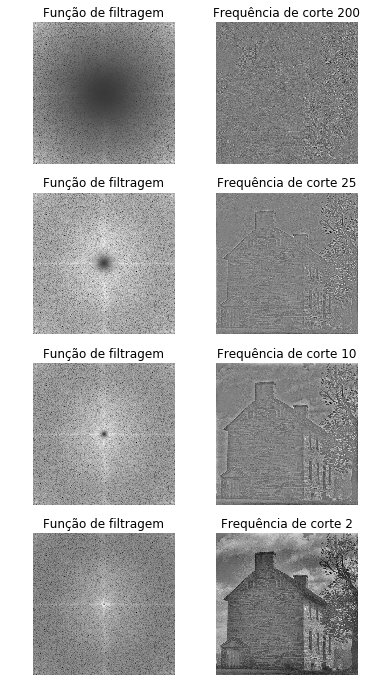
\includegraphics[width=\linewidth]{results/exercicio2passa_alta.png}
    \caption{Passa-alta gaussiano}
    \label{fig:exercicio21}
\end{figure}

\begin{figure}[h!]
    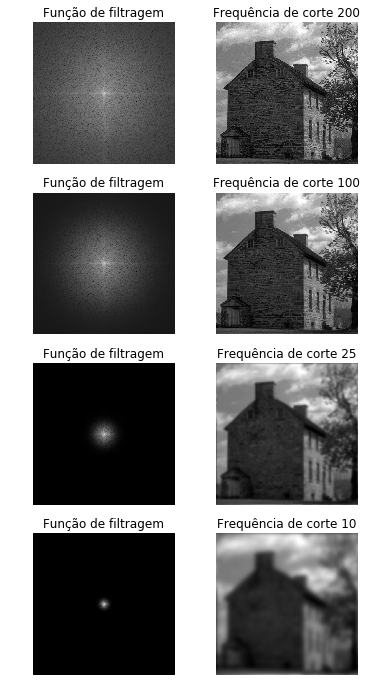
\includegraphics[width=\linewidth]{results/exercicio2passa_baixa.png}
    \caption{Passa-baixa gaussiano}
    \label{fig:exercicio22}
\end{figure}

\begin{figure}[h!]
    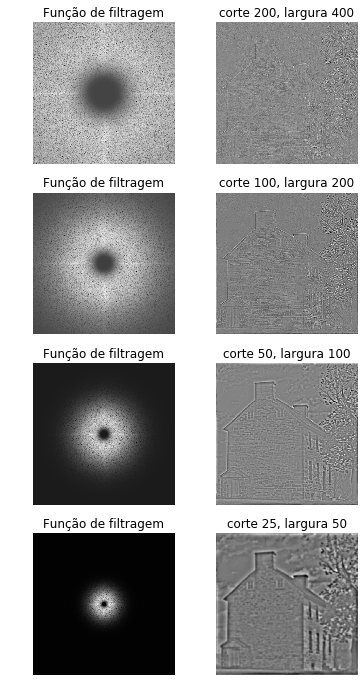
\includegraphics[width=\linewidth]{results/exercicio2passa_faixa.png}
    \caption{Passa-faixa gaussiano}
    \label{fig:exercicio23}
\end{figure}

\begin{figure}[h!]
    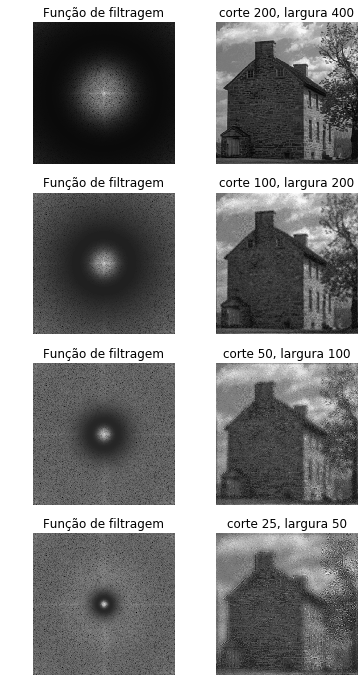
\includegraphics[width=\linewidth]{results/exercicio2rejeita_faixa.png}
    \caption{Rejeita-faixa gaussiano}
    \label{fig:exercicio24}
\end{figure}

\bibliography{relatorio1}
\bibliographystyle{ieeetr}

\end{document}